%!TEX program = xelatex
\documentclass[11pt,article,oneside]{memoir}
\usepackage{org-preamble-xelatex}
\DisemulatePackage{setspace}
\usepackage{setspace}
\usepackage{titling}
\setlength{\droptitle}{-12em}
% \input{vc}


\usepackage{graphicx}
% We will generate all images so they have a width \maxwidth. This means
% that they will get their normal width if they fit onto the page, but
% are scaled down if they would overflow the margins.
\makeatletter
\def\maxwidth{\ifdim\Gin@nat@width>\linewidth\linewidth
\else\Gin@nat@width\fi}
\makeatother
\let\Oldincludegraphics\includegraphics
\renewcommand{\includegraphics}[1]{\Oldincludegraphics[width=\maxwidth]{#1}}

\title{The Early Spread of Mass Media Increases the Probability of Civil War: A
Research Note}

%\author{}

\author{\Large Justin Murphy\vspace{0.05in} \newline\normalsize\emph{University of Southampton} \newline\footnotesize \url{j.murphy@soton.ac.uk}\vspace*{0.2in}\newline }

%\author{Justin Murphy (University of Southampton)}

\date{}


\begin{document}  
\setkeys{Gin}{width=1\textwidth} 	
\setromanfont[Mapping=tex-text,Numbers=OldStyle]{Georgia} 
\setsansfont[Mapping=tex-text]{Gill Sans} 
\setmonofont[Mapping=tex-text,Scale=0.8]{Consolas}
\chapterstyle{article-jmrphy}
\pagestyle{kjh}

\singlespacing


\maketitle



\vspace{-4ex}
\begin{abstract}

\noindent A recent article in \emph{International Organization} suggests that by
enhancing the soft power of states, the spread of mass media decreases
the probability of civil war onset. This research note contributes an
improvement to the logic of that argument (internal consistency) and
demonstrates a substantively different and improved accounting of the
empirical relationship between mass media and civil war (internal and
external validity).

\end{abstract}

\newpage


\onehalfspacing

In a recent issue of \emph{International Organization}, Camber Warren
argues that the spread of mass media technologies throughout a
particular country decreases the probability of observing civil war
because, other things equal, mass media technologies increase state
strength and therefore deter insurgencies. The reason that technologies
such as televisions, radios, and newspapers enhance the state's strength
is because they increase the state's normative influence and therefore
its power to induce loyalty from citizens. More specifically, mass media
technologies increase this ``soft power'' of the state in two ways.

First, mass media technologies lower the costs of communication in
general, for states as well as insurgents. Second, however,mass media
technologies increase the normative influence of the state in particular
because of economies of scale which are unique to the production of
normative influence. Because a media message achieves a larger effect on
receivers who believe the message was widely disseminated, the
production of normative influence through mass media brings increasing
marginal returns for each additional unit of effort, as each additional
recipient receiving the message increases the effect of the message on
the rest of the receivers. Because the state is inherently a
larger-scale producer of symbolic content than potential insurgent
groups, Warren argues, higher levels of mass media will be associated
with normatively stronger states and therefore lower probabilities of
observing civil war.

Grounding this theoretical model in the tradition of figures such as
Karl Deutsche and Benedict Anderson who first diagnosed the role of mass
media in the rise of modern nationalism, as well as contemporary
experimental research on mass-media messaging, Warren's theory stresses
the unique effects of mass communications relative to small-scale
interpersonal communications. Using state-level data for a large panel
of countries from 1945 to 1999, Warren demonstrates that, after
controlling for other predictors of civil war, mass media density
(televisions, radios, and newspapers per person) is associated with more
than a tenfold decrease in the likelihood of observing civil war in a
particular country-year.

But if higher levels of mass media density decrease the likelihood of
civil war, it is extremely puzzling that in modern history, the
international system's most rapid and widespread proliferation of mass
media density has coincided with its most dramatic increases in civil
war. If mass media density decreases the likelihood of civil war as
strongly and robustly as Warren argues, then why has the global
proliferation of mass media since 1945 had no appreciable effect in
pacifying the global prevalence of civil war?

\begin{figure}[htbp]
\centering
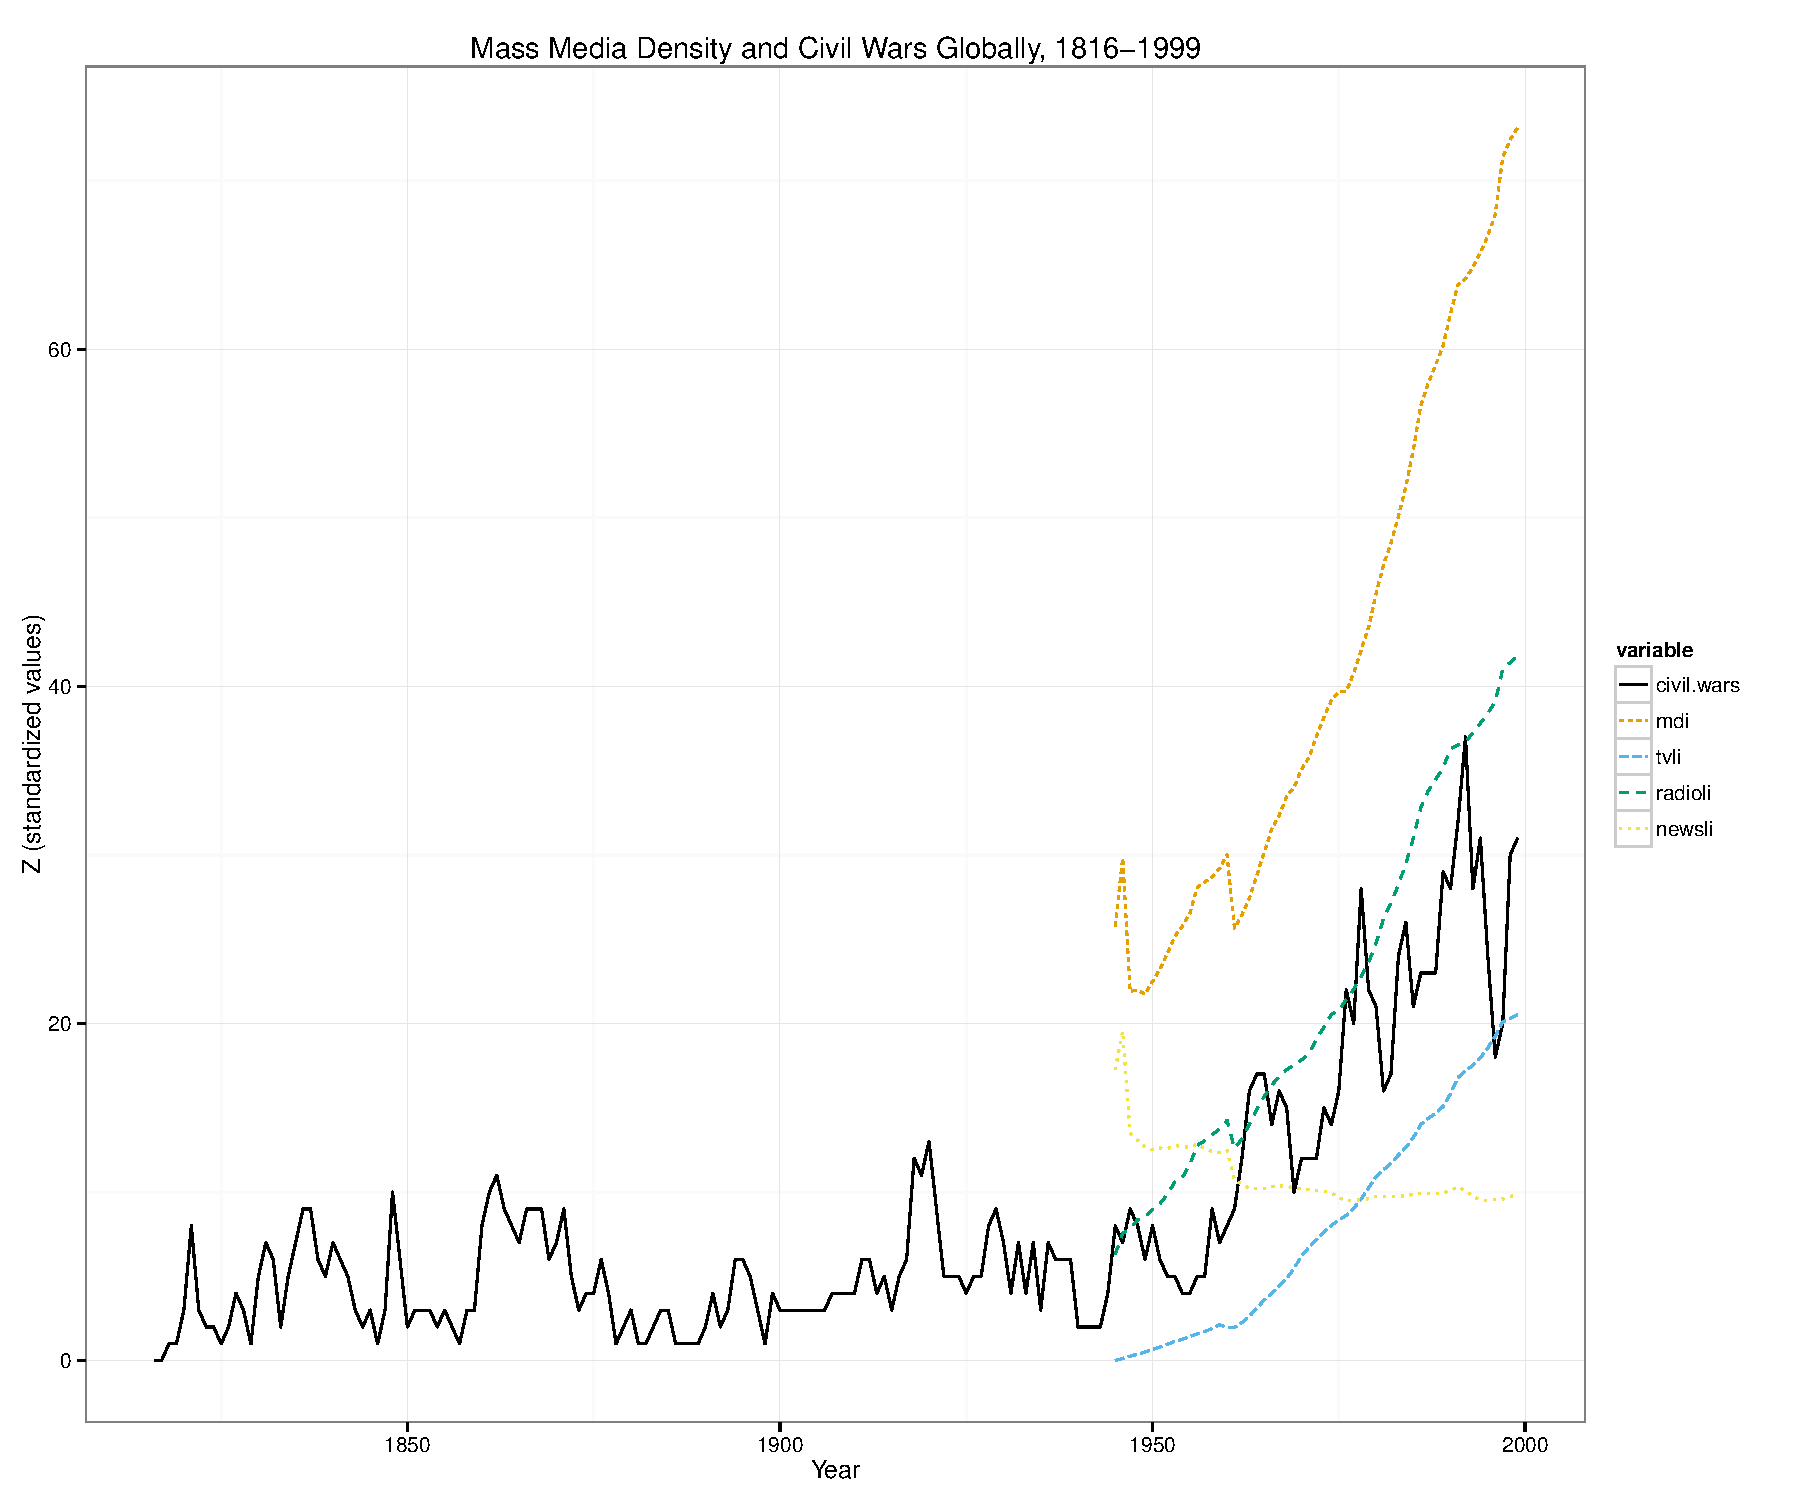
\includegraphics{figure/globalplot.pdf}
\caption{Mass Media Density and Civil Wars Globally, 1816-1999}
\end{figure}

The first shortcoming of Warren's argument is that, while there should
be increasing marginal returns to the production of normative influence
in the context of \emph{mass communications,} there should not be a
linear, one-to-one relationship between a country's mass media density
and its capacity for mass communications. When only a very small
proportion of the population has access to mass media technologies,
those technologies do not imply the presence of a mass communications
system at merely low levels; they imply a country which still
categorically lacks the infrastructural capacity for properly mass
communications.\footnote{Of course, there is no way to know \emph{a
  priori} how many people need access to mass media technologies before
  they constitute a mass public network and therefore the categorical
  presence of a mass communications system. In any event, the question
  is pursued empirically below. At this stage, it suffices simply to
  note the contention that very low levels of mass media density do not
  reflect the positive presence of a mass communications capacity.} If
only a very small proportion of a population has access to television,
radio, or a newspaper, recipients of mass media messaging will know that
the vast majority of others will not be affected by the message. Thus,
within the subset of countries characterized by very low levels of media
density, the normative influence of messages delivered by mass media
technologies should not be enhanced by increasing marginal returns as
these are contingent on the recipient believing the message to be
\emph{widely} spread.

Mass media density only captures the reach of mass communications within
a particular country beyond the threshold at which mass media
technologies are sufficiently widespread to effectively consititute a
mass public network.\footnote{I assume throughout that mass media
  typically first appears within countries at very low levels relative
  to the population (low media density). I also assume throughout that,
  despite variable rates of change and short-run decreases, media
  density has a long-run tendency to increase. In other words, I assume
  that the dynamics of media density are non-stationary and trend
  upward. The Levin-Lin-Chu (2002) and Im-Pesaran-Shin (2003) tests for
  stationarity in panel data fail to reject the null hypothesis that
  media density is non-stationary (p = 0.75 and p = 0.1, respectively).
  See the Appendix for details.}

The second shortcoming is that if the level of mass media \emph{in
general} increases state strength as Warren argues, then for this very
reason, the \emph{first appearance and early growth} of mass media
within a country should increase the utility of controlling the state
relative to other means of merely influencing it. Especially given that
mass media density is non-stationary and trends upward in every country
in which it has been introduced, the first appearance of mass media
technology should increase the incentives of opposition groups to risk
insurgency before the development of a mass communications system
significantly increases the power of the incumbent and decreaes the
power of opposition groups outside the state. Additionally, the closer a
country's mass media density is to the threshold at which it will
constitute a capacity for mass communcations, the more attractive it
will be for opposition groups outside the state to gain control of the
state. It is increasingly urgent as the state becomes nearer to
consolidating its normative domination via mass communications and
therefore significantly less vulnerable to insurgency; also, the closer
the country is to the threshold the less time will a successful
insurgency be vulnerable to yet another insurgency before it
consolidates its own normative consolidation via mass communications.
Thus, if it is true that increasing mass media density makes state power
increasingly safe from insurgency, then before media density crosses the
threshold of constituting mass communications power, \emph{each
increase} in mass media density should further increase the payoffs to
violent insurgency.

This research note advances a different theory of the relationship
between mass media technology and civil war: the \emph{introduction and
early growth} of mass media density within a country \emph{increases}
rather than decreases the likelihood of civil war. Precisely because a
capacity for mass communications increases state power and becomes a
robust deterrent against insurgents, but low levels of mass media
density do not yet constitute that power, year-to-year increases in mass
media density up to a certain threshold should be positively associated
with civil war onset.\footnote{It stands to reason that the same logic
  characterizes the incentives of incumbents, as each increase in mass
  media density up to that threshold also increases the utility of
  defeating insurgencies relative to stepping down or sharing power,
  thus further predicting civil war onsets. Yet the calculus of
  incumbents is likely more complicated given that under certain
  conditions it could be preferable to share the state's new mass
  communications power rather than risk losing it. At present, I focus
  on the calculus of insurgents and leave the calculus of incumbents to
  future research.} It is only beyond that threshold that Warren's
finding of a negative relationship between mass media density and civil
war should hold.

To test whether this theory explains the empirical record better than
Warren's highly parsimonious theory, I pursue a strategy of increasing
causal leverage relative to the original analyses (G King, Keohane, and
Verba 1994, 30). First, I deduce different and more numerous observable
implications for my theory, which provide more numerous opportunities
for falsification. Second, I increase data-set observations by extending
the original sample.(Brady and Collier 2010, 184; G King, Keohane, and
Verba 1994, 30).

\%\%\%\% Front-load emmpirical findings here

\%\%\%\% Sketch importance and implications here

\%\%\%\% Outline the rest of the article here

\section{Review Warren, situated by Deutsche and
Anderson}\label{review-warren-situated-by-deutsche-and-anderson}

\section{Theory}\label{theory}

\begin{itemize}
\itemsep1pt\parskip0pt\parsep0pt
\item
  observable implication 1: differenced mdi in lowest subset
  --\textgreater{} civil war
\item
  observable implication 2: tv and newspapers larger effect in lowest
  subset
\item
  observable implication 3: civil war more likely after 1945 than before
\end{itemize}

\section{Analysis}\label{analysis}

All models use rare-events logistic regression.\footnote{Traditional
  logistic regression estimated by maximum-likelihood would likely
  underestimate the probability of civil war onsets because civil wars
  begin in relatively very few country-years (Gary King and Zeng 2001).
  There are 119 (2.06\%) onsets in the full sample and 63 (3.47\%) in
  the subset of low-MDI country years.}

\begin{figure}[htbp]
\centering
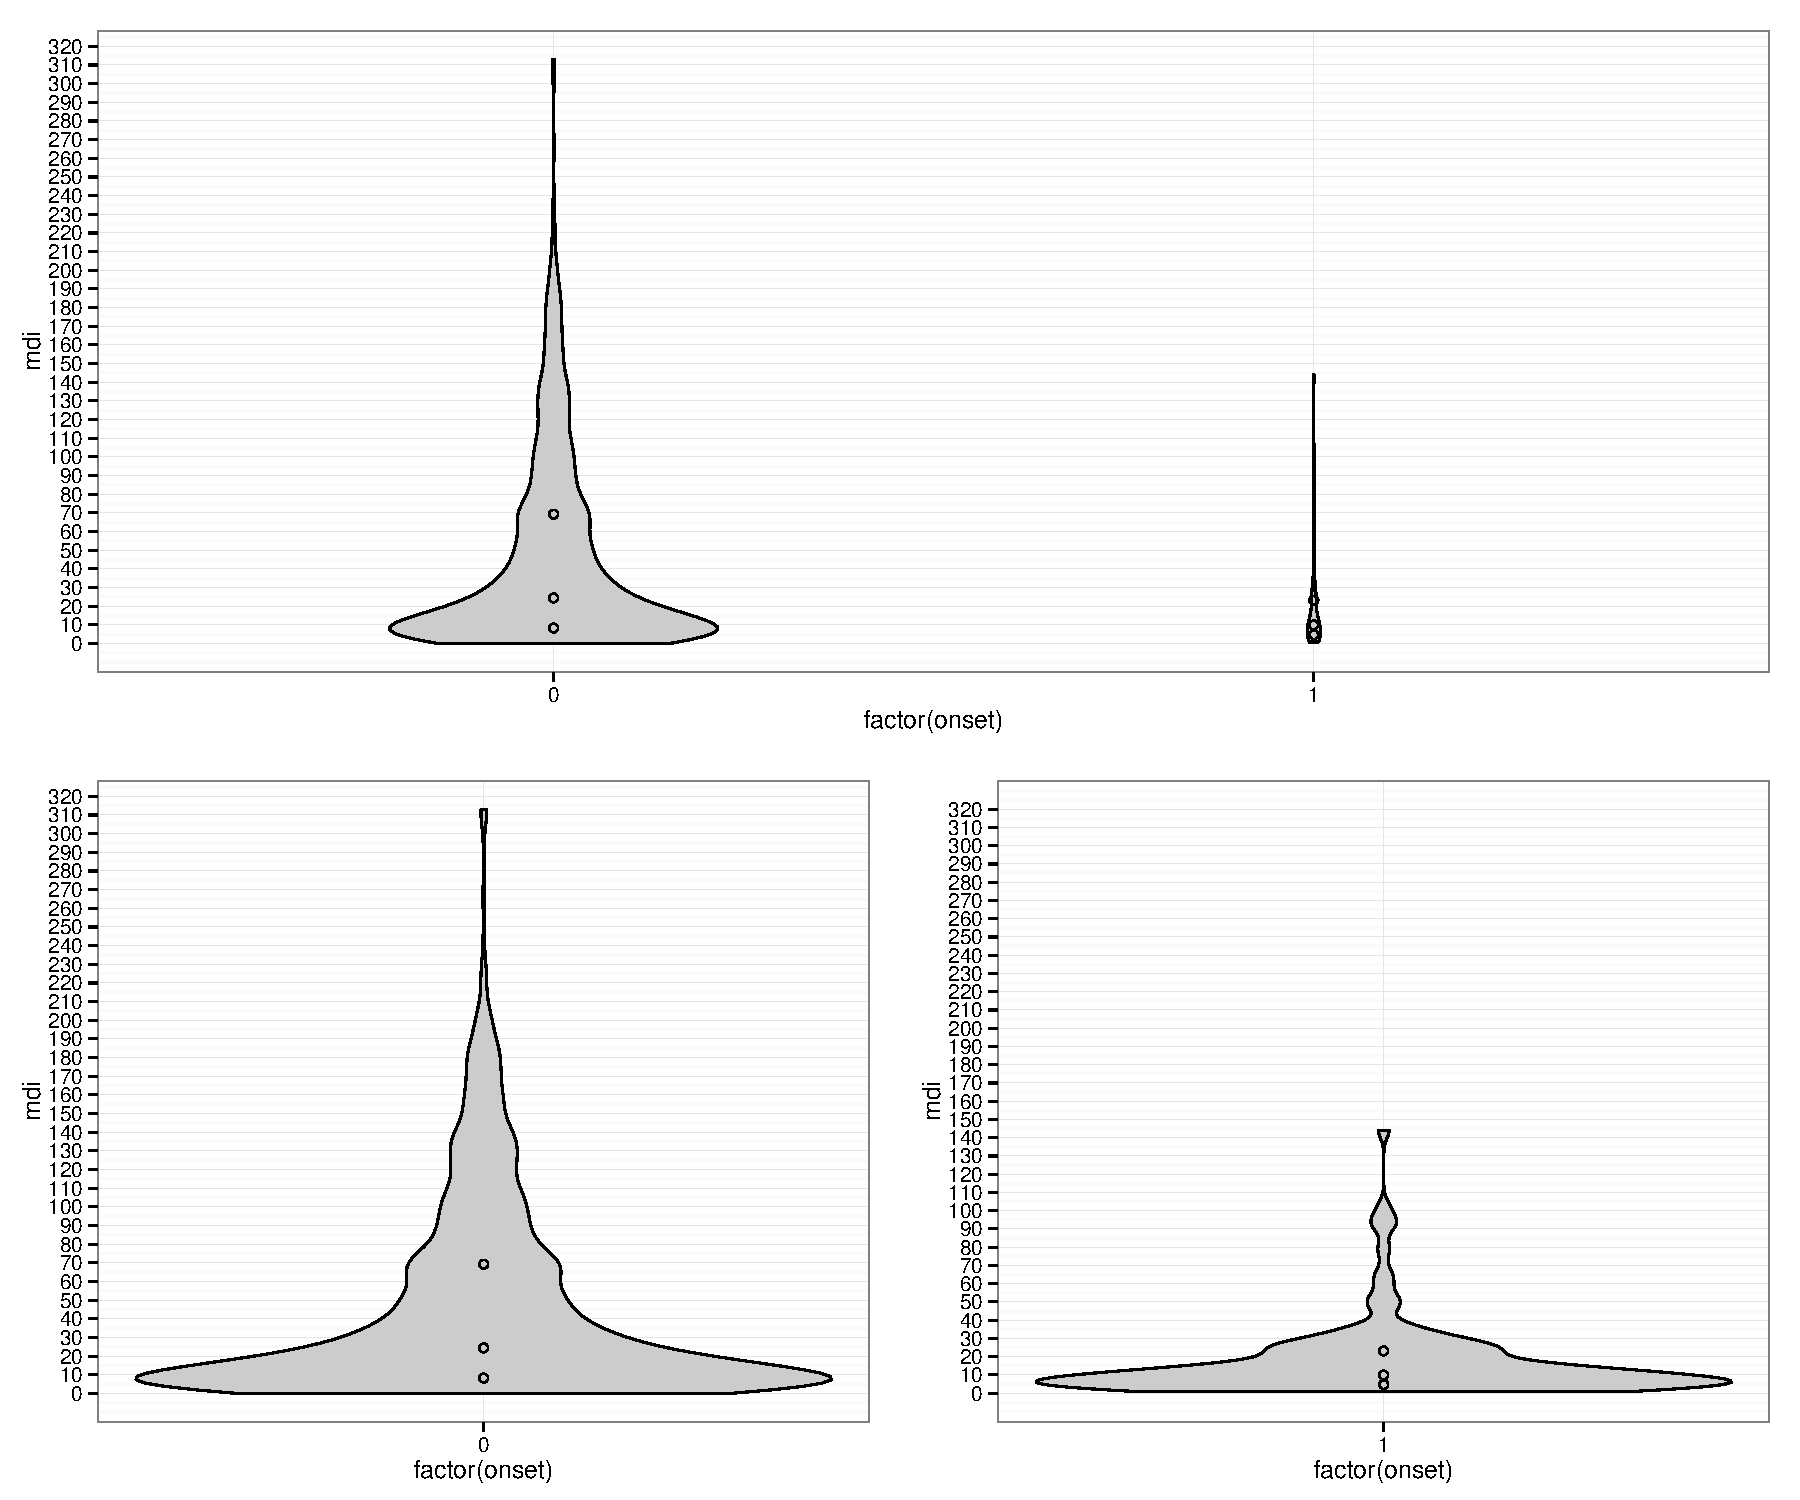
\includegraphics{figure/violinplot.pdf}
\caption{Violin plot of media density for all civil war onsets}
\end{figure}

\begin{table}[!htbp] \centering 
  \caption{Early Growth of Media Density Compared to Media Density in General} 
  \label{} 
\footnotesize 
\begin{tabular}{@{\extracolsep{5pt}}lccc} 
\\[-1.8ex]\hline \\[-1.8ex] 
 & Warren & \multicolumn{2}{c}{Low MDI} \\ 
\\[-1.8ex] & (1) & (2) & (3)\\ 
\hline \\[-1.8ex] 
 MDI & $-$2.60$^{***}$ &  &  \\ 
  & (0.71) &  &  \\ 
  $\Delta$MDI &  & 0.48$^{**}$ &  \\ 
  &  & (0.24) &  \\ 
  $\Delta$NEWSPAPER &  &  & 1.40$^{*}$ \\ 
  &  &  & (0.75) \\ 
  $\Delta$RADIO &  &  & 0.27 \\ 
  &  &  & (0.31) \\ 
  $\Delta$TV &  &  & 2.10$^{*}$ \\ 
  &  &  & (1.20) \\ 
  GDP PER CAPITA & $-$0.09 & $-$0.56 & $-$0.49 \\ 
  & (0.36) & (0.36) & (0.31) \\ 
  AREA & $-$0.31 & 0.02 & 0.001 \\ 
  & (0.32) & (0.42) & (0.15) \\ 
  MOUNTAINOUS TERRAIN & 0.45$^{*}$ & 0.48 & 0.11 \\ 
  & (0.24) & (0.36) & (0.09) \\ 
  POPULATION & 0.80$^{***}$ & 0.79$^{**}$ & 0.28$^{**}$ \\ 
  & (0.25) & (0.36) & (0.13) \\ 
  OIL EXPORTER & 0.76$^{***}$ & 1.10$^{**}$ & 1.20$^{**}$ \\ 
  & (0.28) & (0.47) & (0.48) \\ 
  DEMOCRACY & 2.70$^{**}$ & 2.60$^{*}$ & 0.23$^{*}$ \\ 
  & (1.10) & (1.30) & (0.12) \\ 
  DEMOCRACY$^2$ & $-$2.50$^{**}$ & $-$2.00 & $-$0.01 \\ 
  & (1.20) & (1.30) & (0.01) \\ 
  ETHNIC FRACTIONALIZATION & 0.11 & $-$0.43 & $-$0.59 \\ 
  & (0.21) & (0.32) & (0.55) \\ 
  RELIGIOUS FRACTIONALIZATION & 0.60$^{***}$ & 0.53 & 1.40$^{*}$ \\ 
  & (0.23) & (0.33) & (0.79) \\ 
  PEACE YEARS & $-$1.90 & $-$2.00 & $-$0.10 \\ 
  & (2.60) & (2.50) & (0.12) \\ 
  SPLINE 1 & $-$0.55 & $-$6.10 & $-$0.002 \\ 
  & (16.00) & (12.00) & (0.003) \\ 
  SPLINE 2 & $-$5.20 & 3.50 & 0.0004 \\ 
  & (18.00) & (14.00) & (0.001) \\ 
  SPLINE 3 & 3.50 & 0.20 & $-$0.0000 \\ 
  & (5.60) & (4.00) & (0.0003) \\ 
  CONSTANT & $-$4.50$^{***}$ & $-$3.80$^{***}$ & $-$9.70$^{***}$ \\ 
  & (0.18) & (0.20) & (1.80) \\ 
 \textit{Observations} & 5,899 & 1,672 & 1,672 \\ 
\textit{Log likelihood} & $-$528.00 & $-$220.00 & $-$218.00 \\ 
\textit{Akaike information criterion} & 1,085.00 & 470.00 & 471.00 \\ 
\hline \\[-1.8ex] 
\textit{Notes:} & \multicolumn{3}{l}{$^{***}$p $<$ .01; $^{**}$p $<$ .05; $^{*}$p $<$ .1} \\ 
\end{tabular} 
\end{table}

\begin{figure}[htbp]
\centering
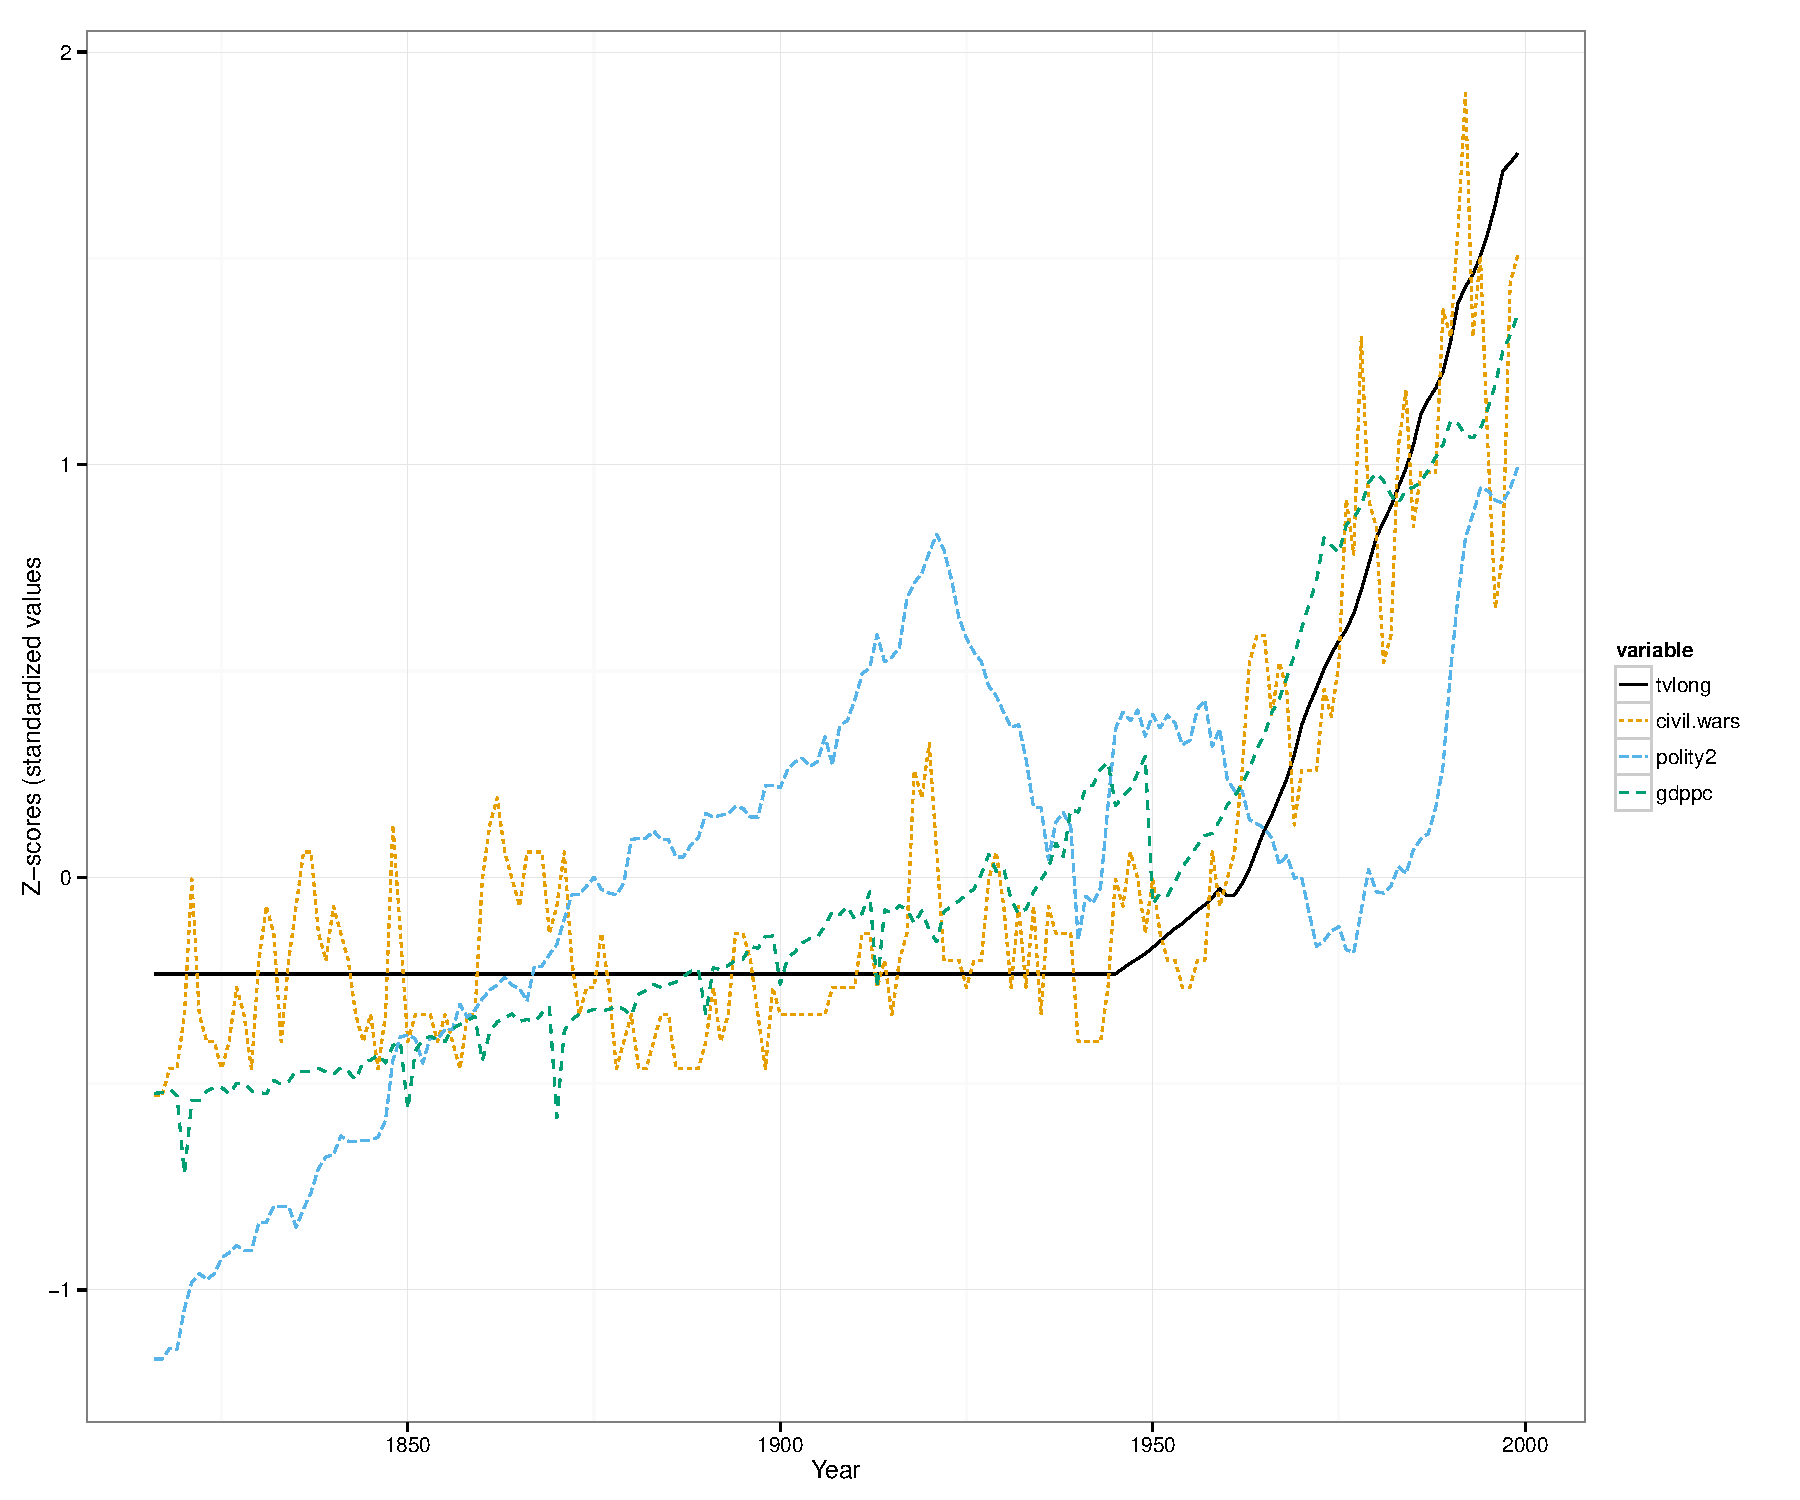
\includegraphics{figure/longrunplot.pdf}
\caption{TV, Democracy, Economic Growth, and Civil Wars Globally,
1816-1999}
\end{figure}

\begin{table}[!htbp] \centering 
  \caption{Historical Regressions} 
  \label{} 
\footnotesize 
\begin{tabular}{@{\extracolsep{5pt}}lc} 
\\[-1.8ex]\hline \\[-1.8ex] 
\\[-1.8ex] & civil.wars \\ 
\hline \\[-1.8ex] 
 TV & $-$0.37$^{**}$ \\ 
  & (0.16) \\ 
  $\Delta$TV & 2.20$^{*}$ \\ 
  & (1.30) \\ 
  GDP PER CAPITA & $-$0.03 \\ 
  & (0.18) \\ 
  $\Delta$GDP PER CAPITA & 0.32 \\ 
  & (0.33) \\ 
  DEMOCRACY & $-$0.09 \\ 
  & (0.09) \\ 
  DEMOCRACY$^2$ & $-$1.20$^{***}$ \\ 
  & (0.25) \\ 
  CIVIL WARS$_{t-1}$ & 0.09$^{***}$ \\ 
  & (0.01) \\ 
  $\Delta$CIVIL WARS & 0.09$^{***}$ \\ 
  & (0.01) \\ 
  YEAR & 0.002 \\ 
  & (0.002) \\ 
  CONSTANT & $-$4.80$^{**}$ \\ 
  & (2.40) \\ 
 \textit{Observations} & 181 \\ 
\textit{Log likelihood} & $-$376.00 \\ 
$\theta$ & 186,980.00  (1,919,136.00) \\ 
\textit{Akaike information criterion} & 772.00 \\ 
\hline \\[-1.8ex] 
\textit{Notes:} & \multicolumn{1}{l}{$^{***}$p $<$ .01; $^{**}$p $<$ .05; $^{*}$p $<$ .1} \\ 
\end{tabular} 
\end{table}

\begin{figure}[htbp]
\centering
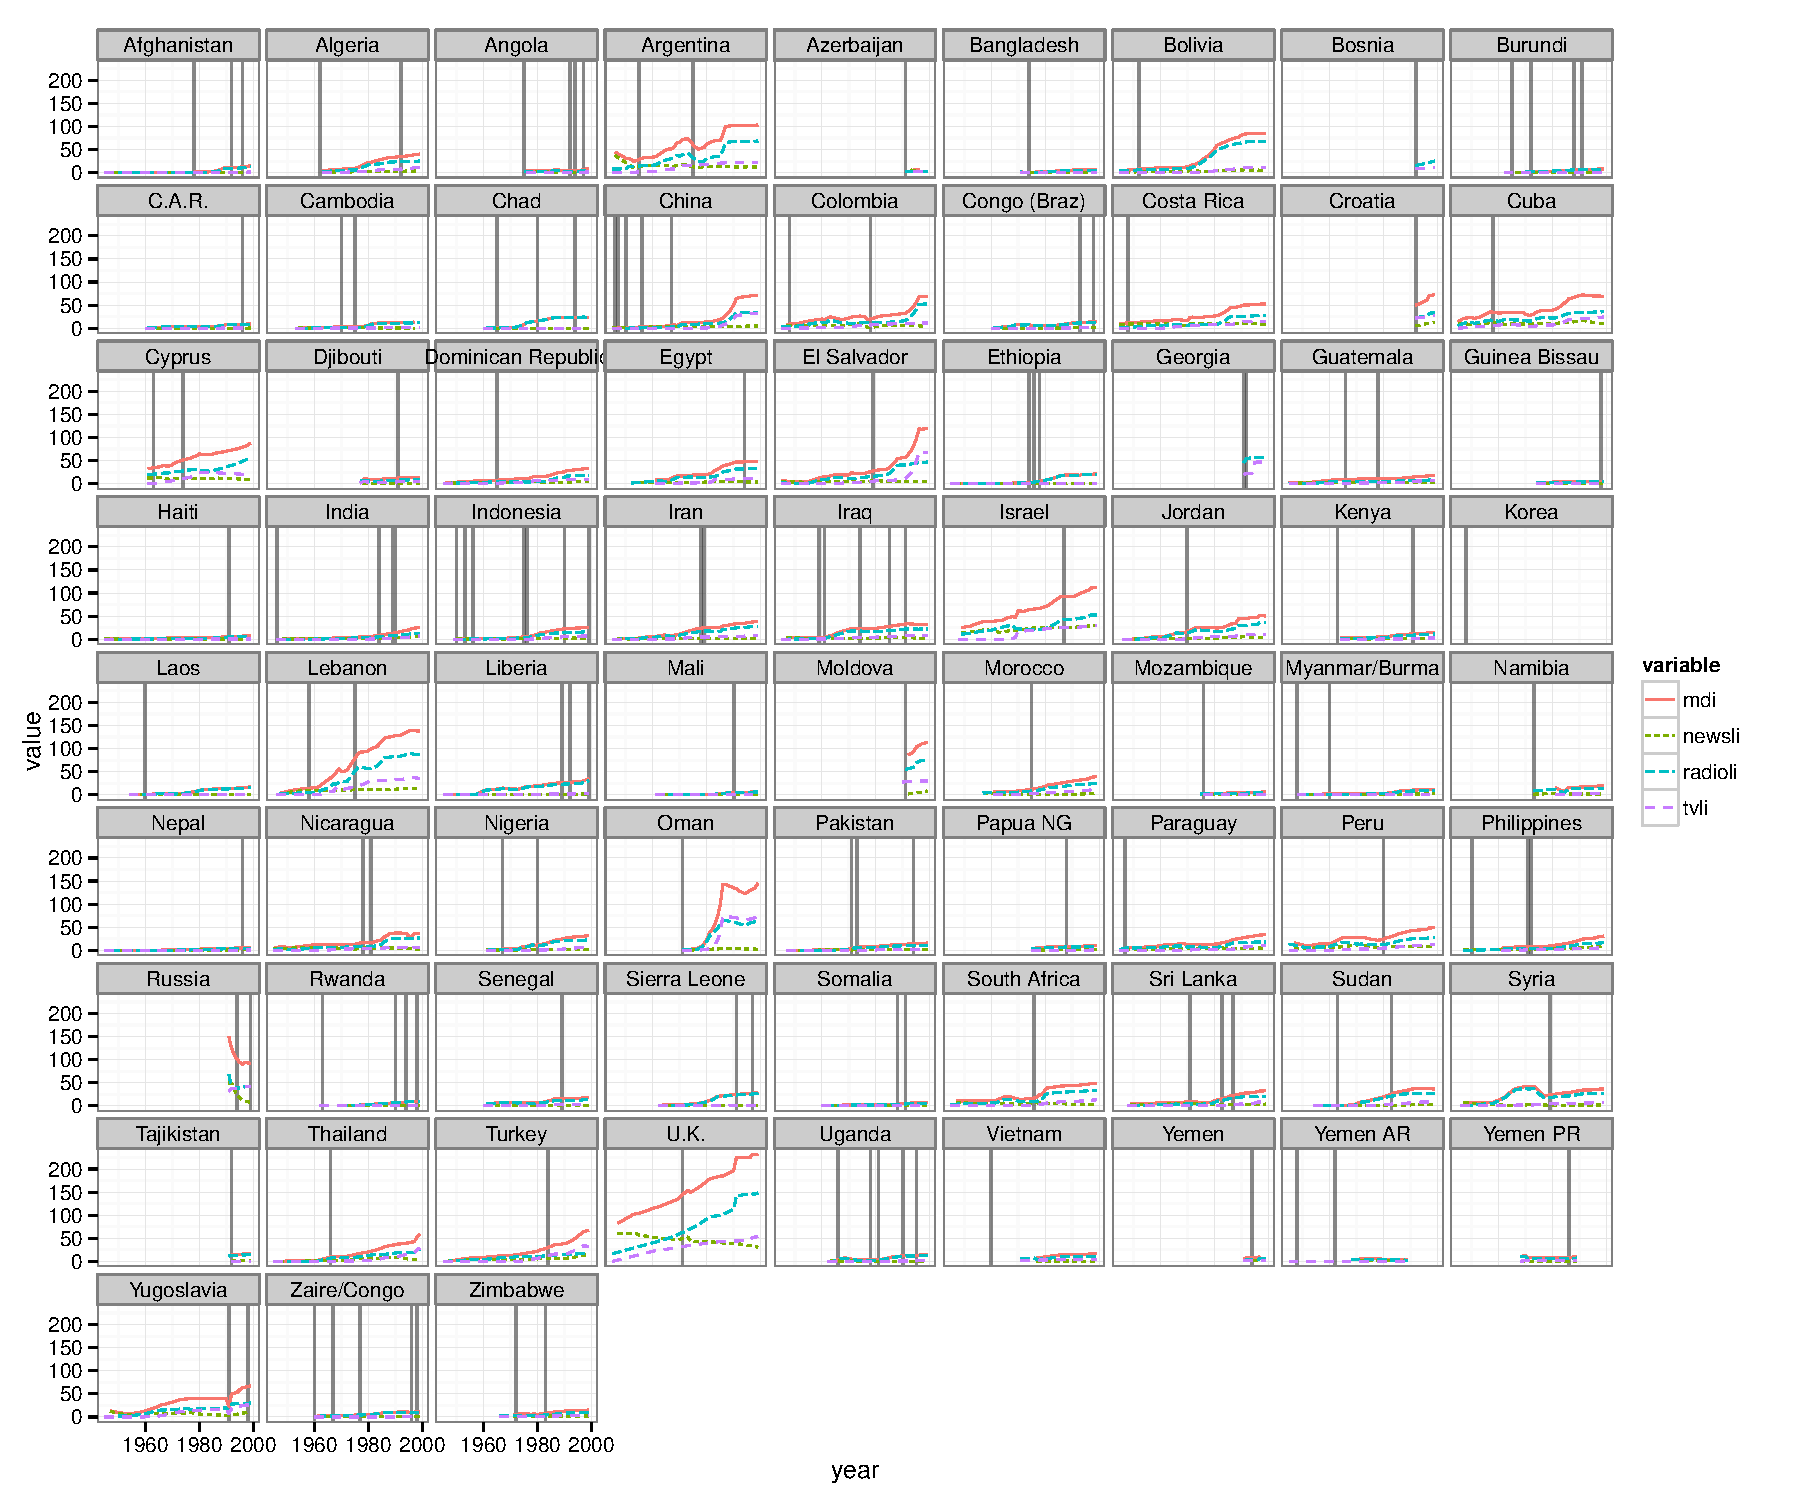
\includegraphics{figure/full_panel_plot.pdf}
\caption{Disaggregated media density and all civil war onsets over time,
by country}
\end{figure}

\section{Conclusion}\label{conclusion}

\section{Appendix}\label{appendix}

The Levin-Lin-Chu statistic is a standard test for the presence of a
unit root, otherwise known as non-stationarity or integration of order
I(1), in a time series variable observed across multiple cross-sectional
units. The Im-Pesaran-Shin test is a ``second generation'' test which is
robust to cross-sectional dependence, common in cross-national panel
data. For each test, the null hypothesis is the presence of a unit root.
Because the tests require balanced panels, they were applied only to the
24 countries with the maximum time-series of 55 years, a subset which
still contains significant variation in geography, income, regime type,
and other factors. Specifically, the countries in this subset are:
Canada, Cuba, Haiti, Dominican Republic, Mexico, Honduras, El Salvador,
Nicaragua, Costa Rica, Uruguay, Ireland, Netherlands, Belgium,
Luxembourg, France, Switzerland, Hungary, Romania, Finland, Sweden,
Norway, Denmark, Afghanistan, China.

\begin{verbatim}
Levin-Lin-Chu Unit-Root Test (ex. var. : Individual Intercepts
and Trend )
\end{verbatim}

data: unit\$mdi z.x1 = -0.32, p-value = 0.7473 alternative hypothesis:
stationarity

\begin{verbatim}
Pesaran's CIPS test for unit roots
\end{verbatim}

data: unit\$mdi CIPS test = -2.1, lag order = 2, p-value = 0.1
alternative hypothesis: Stationarity

\pagebreak   

\section{References}\label{references}

\setlength{\parindent}{-0.2in} \setlength{\leftskip}{0.2in}
\setlength{\parskip}{8pt} \vspace*{-0.2in} \noindent

Brady, Henry E, and David Collier. 2010. \emph{Rethinking Social
Inquiry: Diverse Tools, Shared Standards}. Lanham: Rowman \&
Littlefield. \url{http://books.google.co.uk/books?id=djovjEXZYccC}.

Im, Kyung So, M Hashem Pesaran, and Yongcheol Shin. 2003. ``Testing for
Unit Roots in Heterogeneous Panels.'' \emph{Journal of Econometrics}
115(1): 53--74.
\url{http://linkinghub.elsevier.com/retrieve/pii/S0304407603000927}.

King, G, R O Keohane, and S Verba. 1994. \emph{Designing Social Inquiry:
Scientific Inference in Qualitative Research}. Princeton University
Press. \url{http://books.google.com/books?id=A7VFF-JR3b8C}.

King, Gary, and Langche Zeng. 2001. ``Logistic Regression in Rare Events
Data.'' \emph{Political Analysis} 9(2): 137--63.
\url{http://dash.harvard.edu/bitstream/handle/1/4125045/relogit\%20rare\%20events.pdf?s}.

Levin, Andrew, Chien-Fu Lin, and Chia-Shang James Chu. 2002. ``Unit Root
Tests in Panel Data: Asymptotic and Finite-Sample Properties.''
\emph{Journal of Econometrics} 108(1): 1--24.
\url{http://linkinghub.elsevier.com/retrieve/pii/S0304407601000987}.


\end{document}